\documentclass{beamer}

\usepackage{graphicx}
\usepackage{caption}

\begin{document}
	
	\begin{frame}[plain]
		\begin{figure}
			\centering
			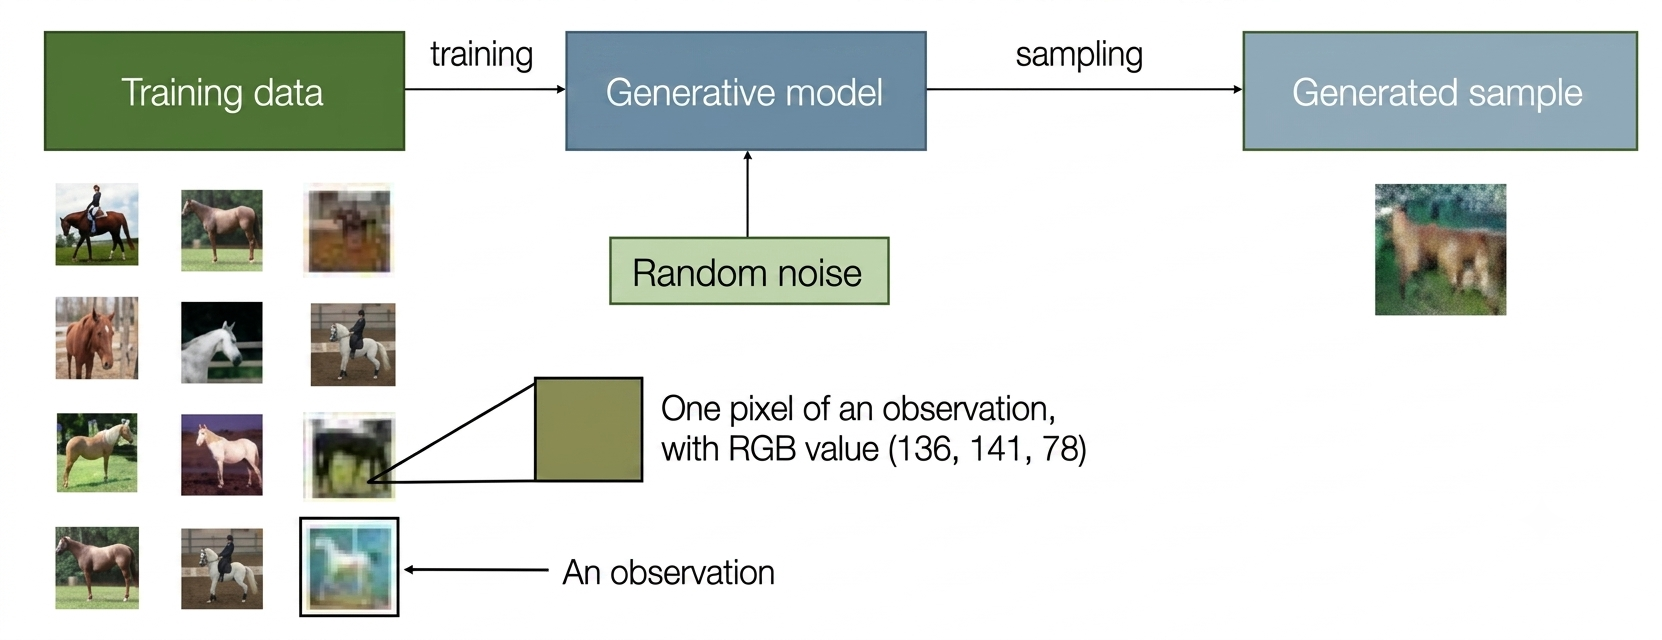
\includegraphics[width=\textwidth,height=0.85\textheight,keepaspectratio]{11.png}
			\caption{The generative modeling process}
		\end{figure}
	\end{frame}
	
	\begin{frame}[plain]
		\begin{figure}
			\centering
			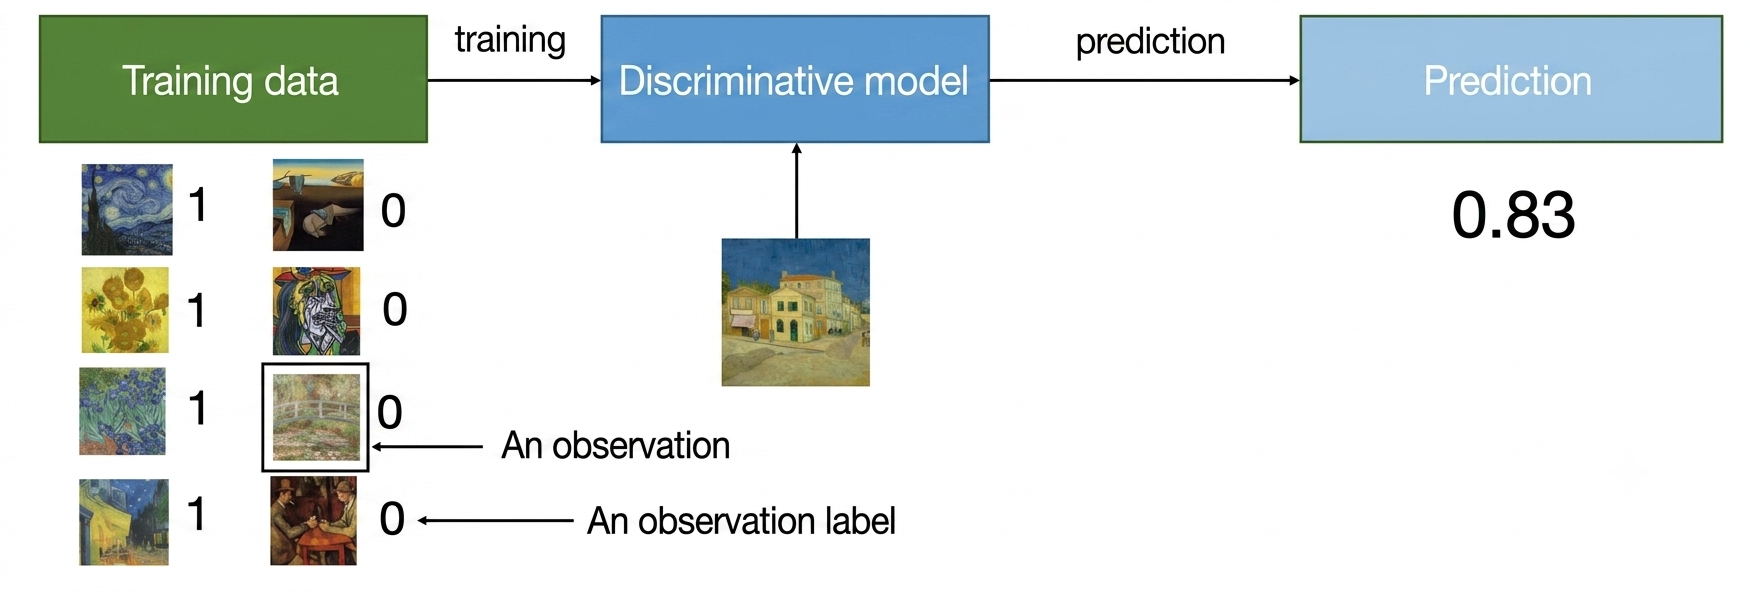
\includegraphics[width=\textwidth,height=0.85\textheight,keepaspectratio]{12.png}
			\caption{The discriminative modeling process}
		\end{figure}
	\end{frame}
	
	\begin{frame}[plain]
		\begin{figure}
			\centering
			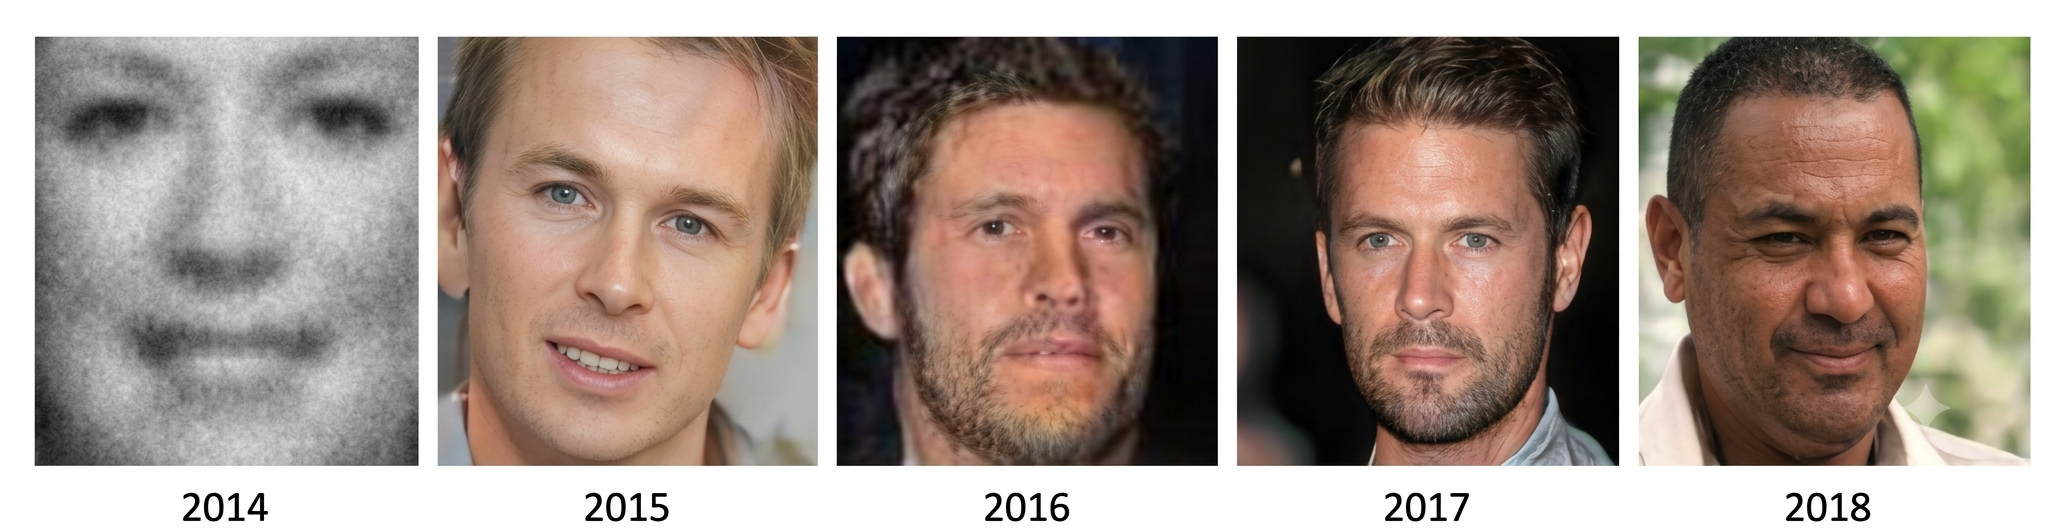
\includegraphics[width=\textwidth,height=0.85\textheight,keepaspectratio]{13.png}
			\caption{Face generation using generative modeling has improved significantly in the
				last four years}
		\end{figure}
	\end{frame}
	
	\begin{frame}[plain]
		\begin{figure}
			\centering
			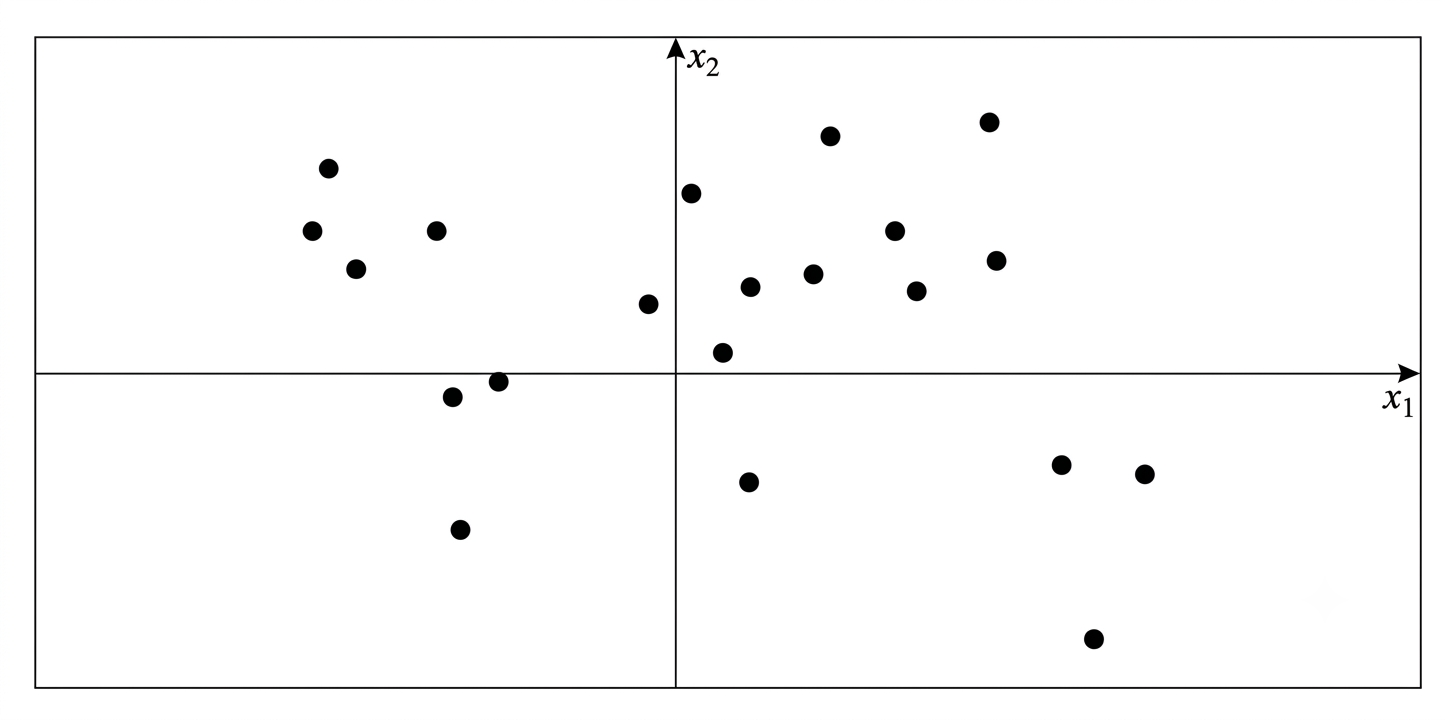
\includegraphics[width=\textwidth,height=0.85\textheight,keepaspectratio]{14.png}
			\caption{A set of points in two dimensions, generated by an unknown rule $p_{\mathrm{data}}$}
		\end{figure}
	\end{frame}
	
	\begin{frame}[plain]
		\begin{figure}
			\centering
			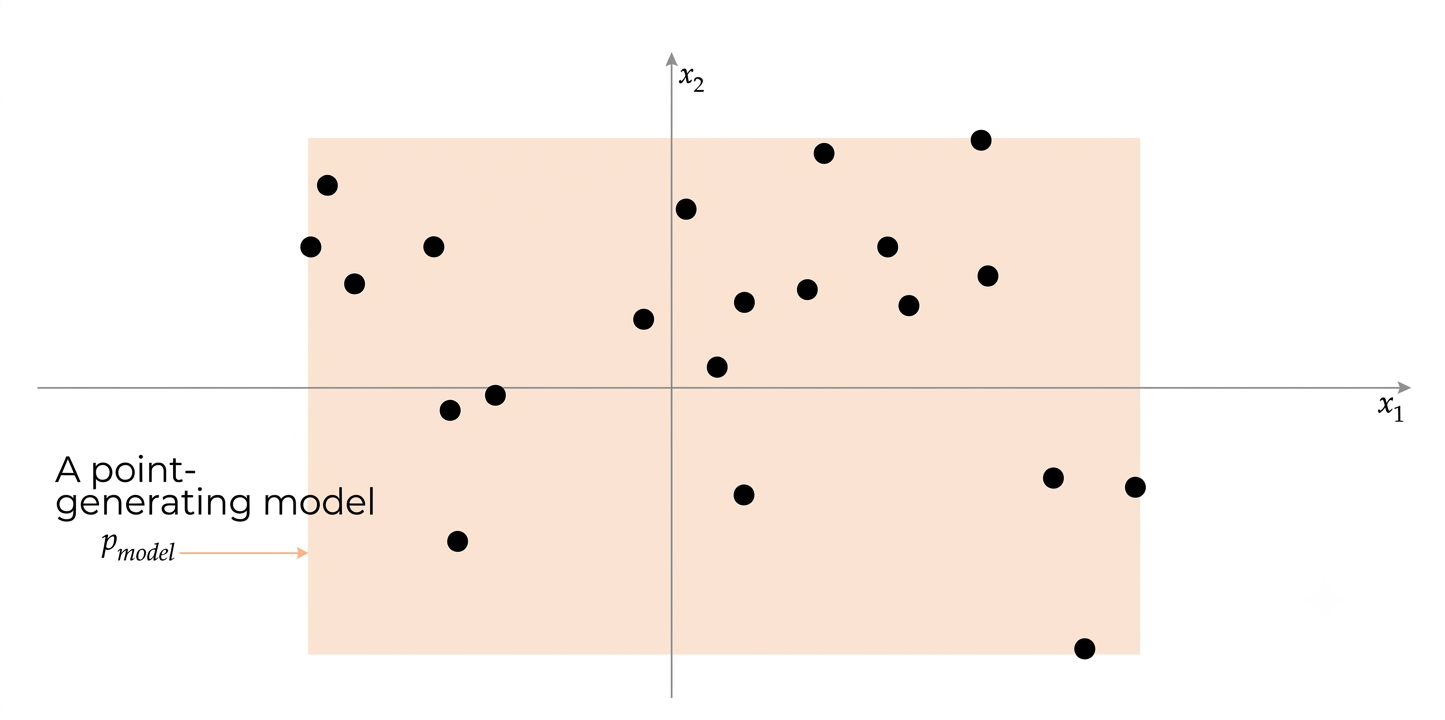
\includegraphics[width=\textwidth,height=0.85\textheight,keepaspectratio]{15.png}
			\caption{The orange box, $p_{\text{model}}$, is an estimate of the true data-generating distribution, $p_{\text{data}}$.}
		\end{figure}
	\end{frame}
	
	\begin{frame}[plain]
		\begin{figure}
			\centering
			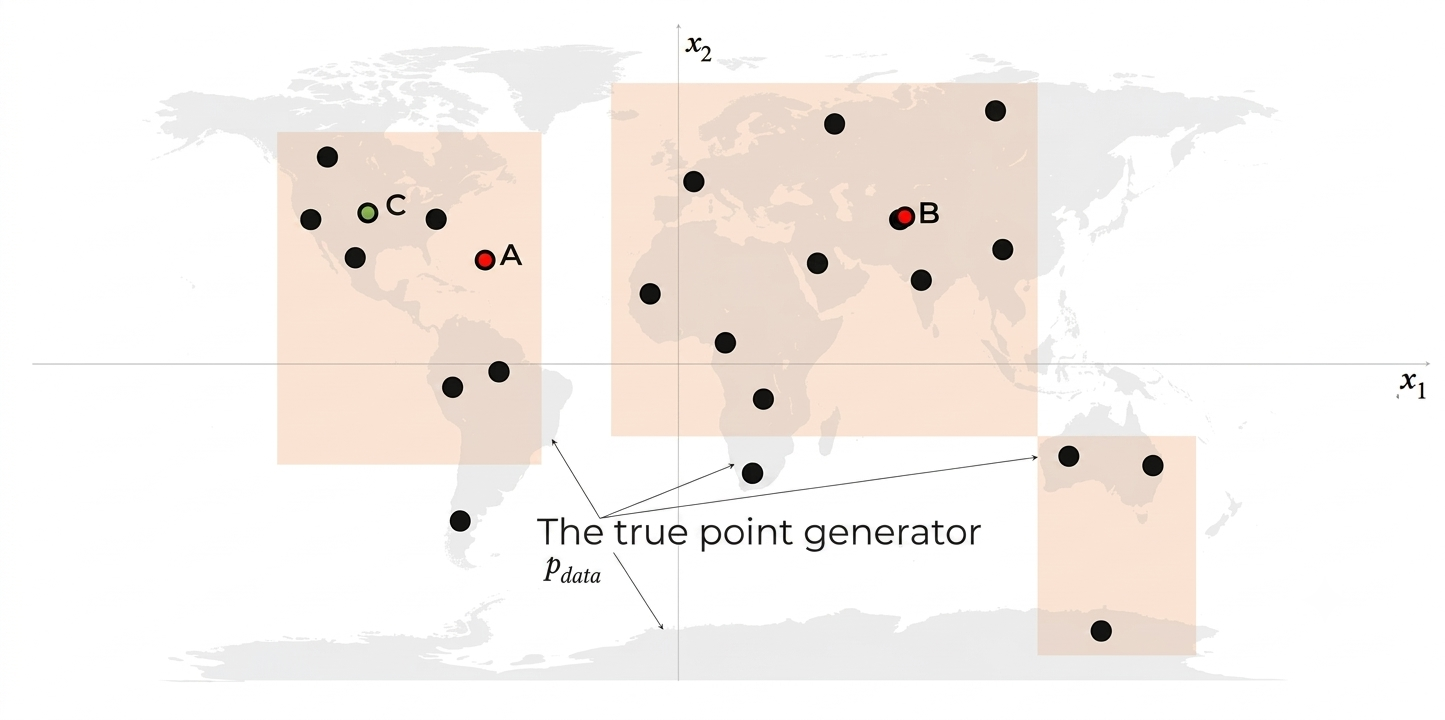
\includegraphics[width=\textwidth,height=0.85\textheight,keepaspectratio]{16.png}
			\caption{The orange box, $p_{\text{model}}$, is an estimate of the true data-generating distribution, $p_{\text{data}}$ (the gray area).}
		\end{figure}
	\end{frame}
	
	\begin{frame}[plain]
		\begin{figure}
			\centering
			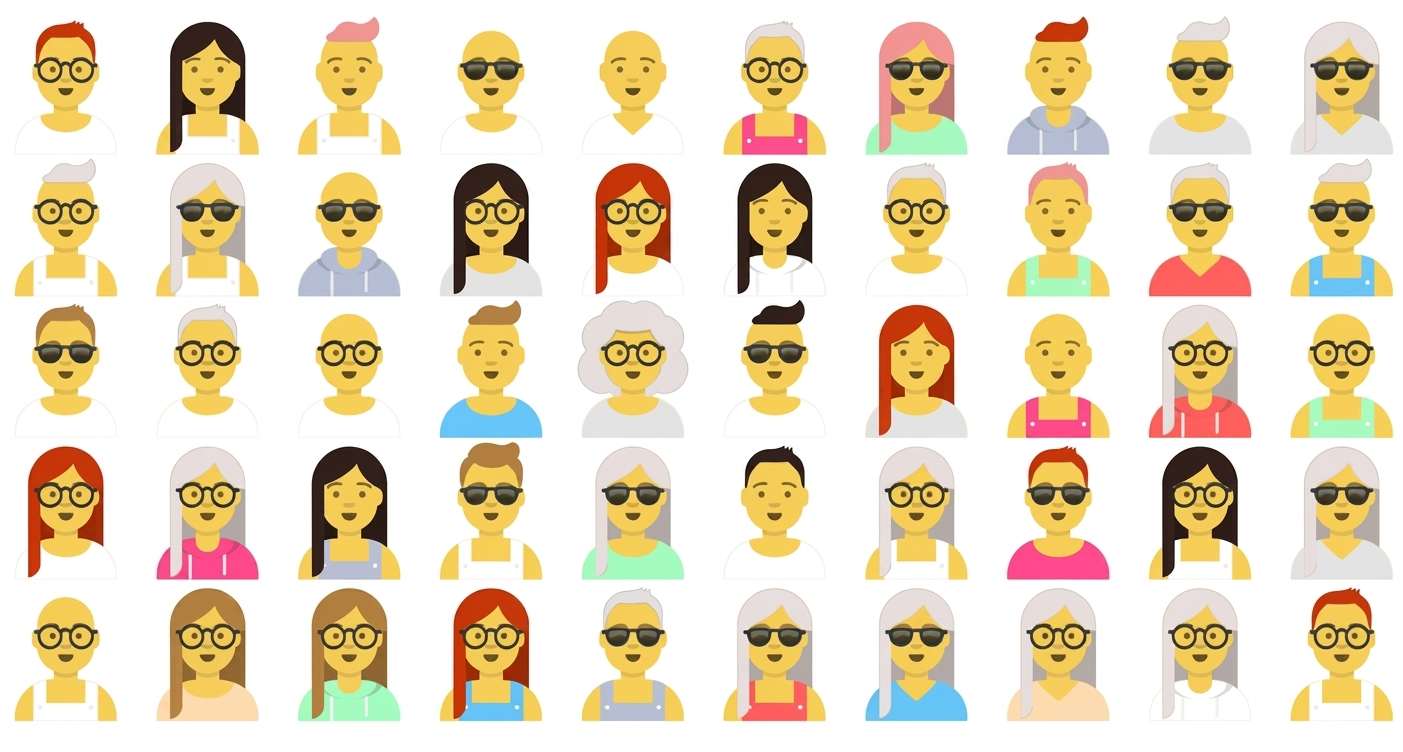
\includegraphics[width=\textwidth,height=0.85\textheight,keepaspectratio]{17.png}
			\caption{Headshots of 50 Wrodlers}
		\end{figure}
	\end{frame}
	
	\begin{frame}[plain]
		\begin{figure}
			\centering
			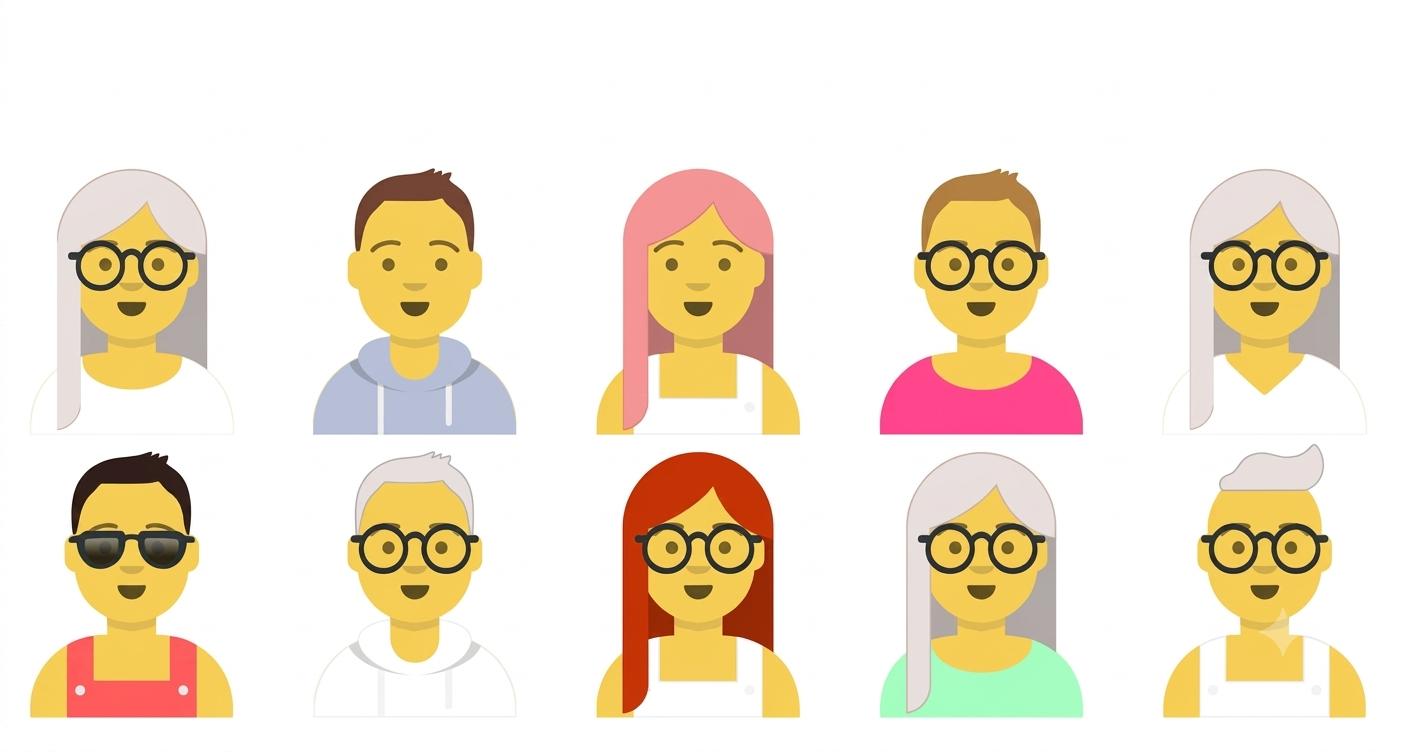
\includegraphics[width=\textwidth,height=0.85\textheight,keepaspectratio]{18.png}
			\caption{Ten new Wrodl styles, generated using the Naive Bayes model}
		\end{figure}
	\end{frame}
	
	\begin{frame}[plain]
		\begin{figure}
			\centering
			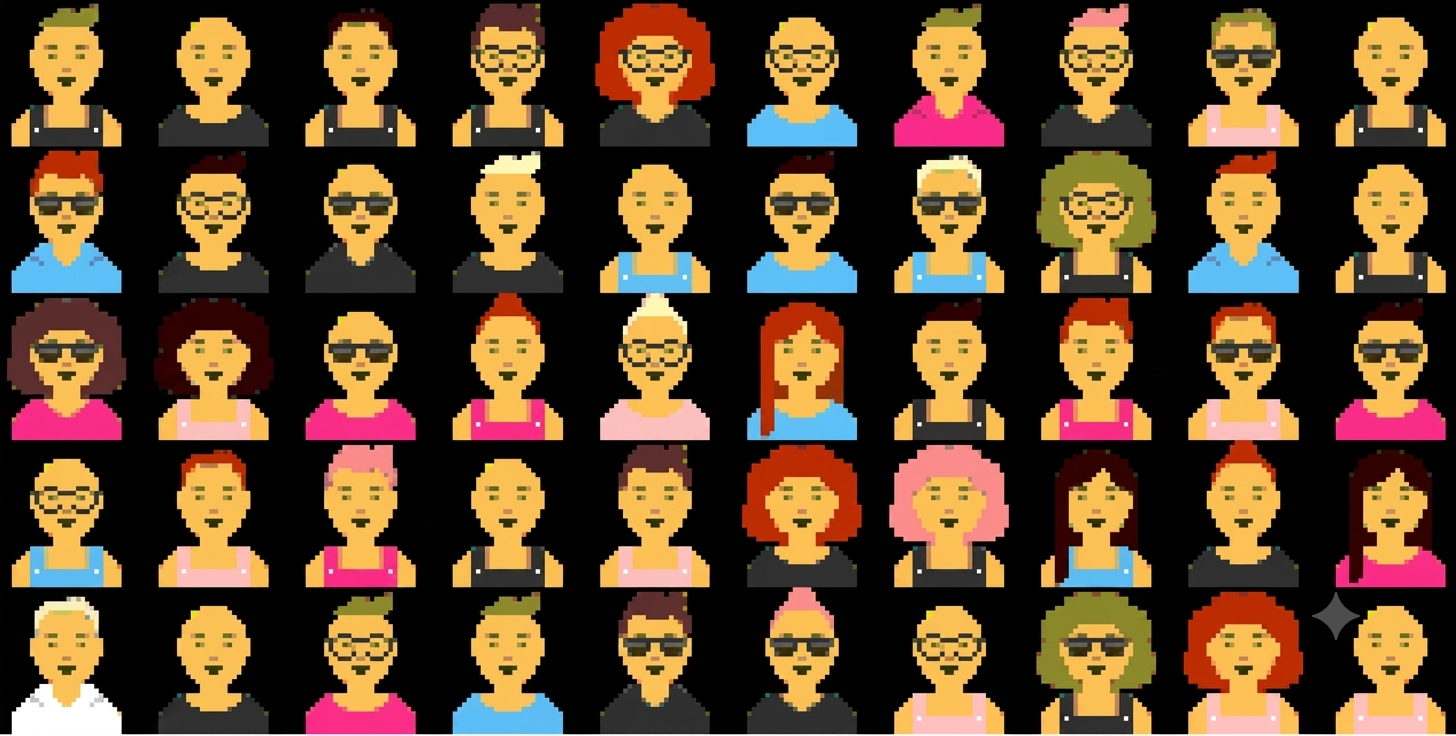
\includegraphics[width=\textwidth,height=0.85\textheight,keepaspectratio]{19.png}
			\caption{Fashions on Planet Pixel}
		\end{figure}
	\end{frame}
	
	\begin{frame}[plain]
		\begin{figure}
			\centering
			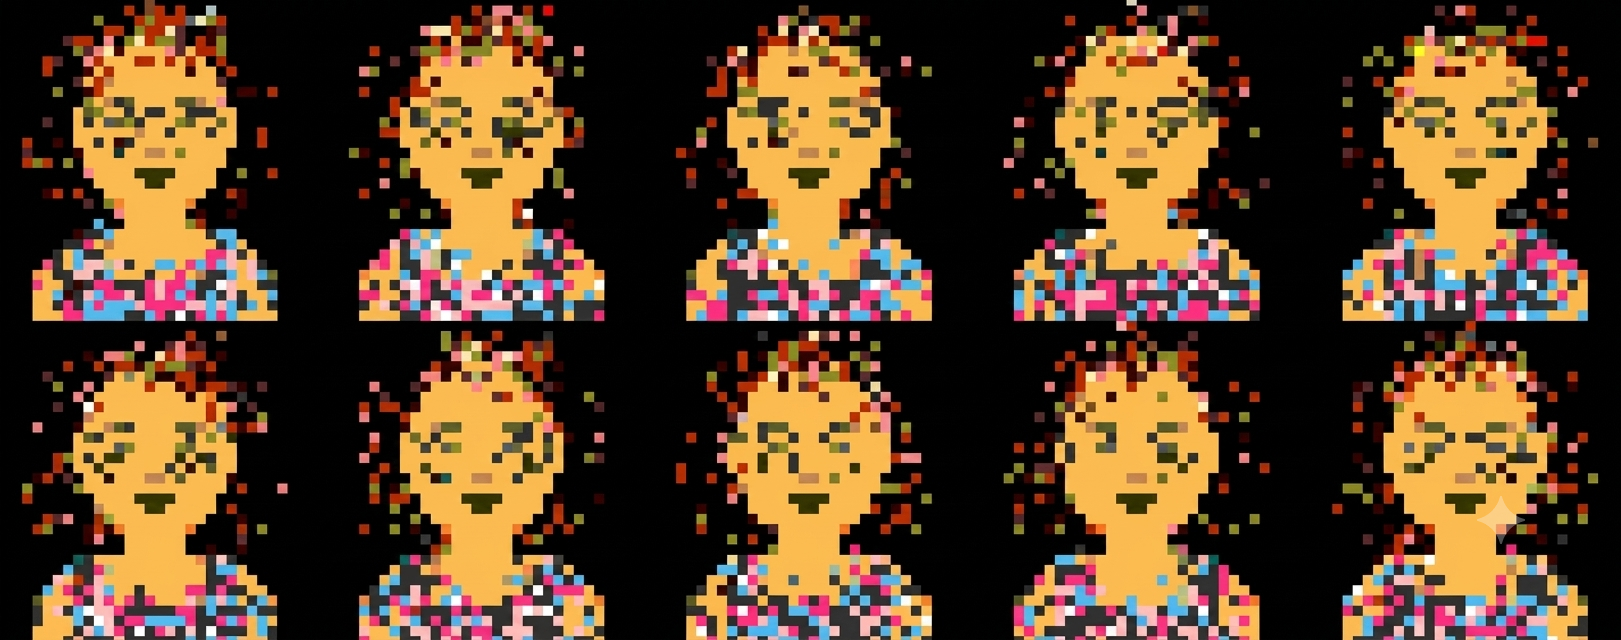
\includegraphics[width=\textwidth,height=0.85\textheight,keepaspectratio]{110.png}
			\caption{Ten new Planet Pixel styles, generated by the Naive Bayes model}
		\end{figure}
	\end{frame}
	
	\begin{frame}[plain]
		\begin{figure}
			\centering
			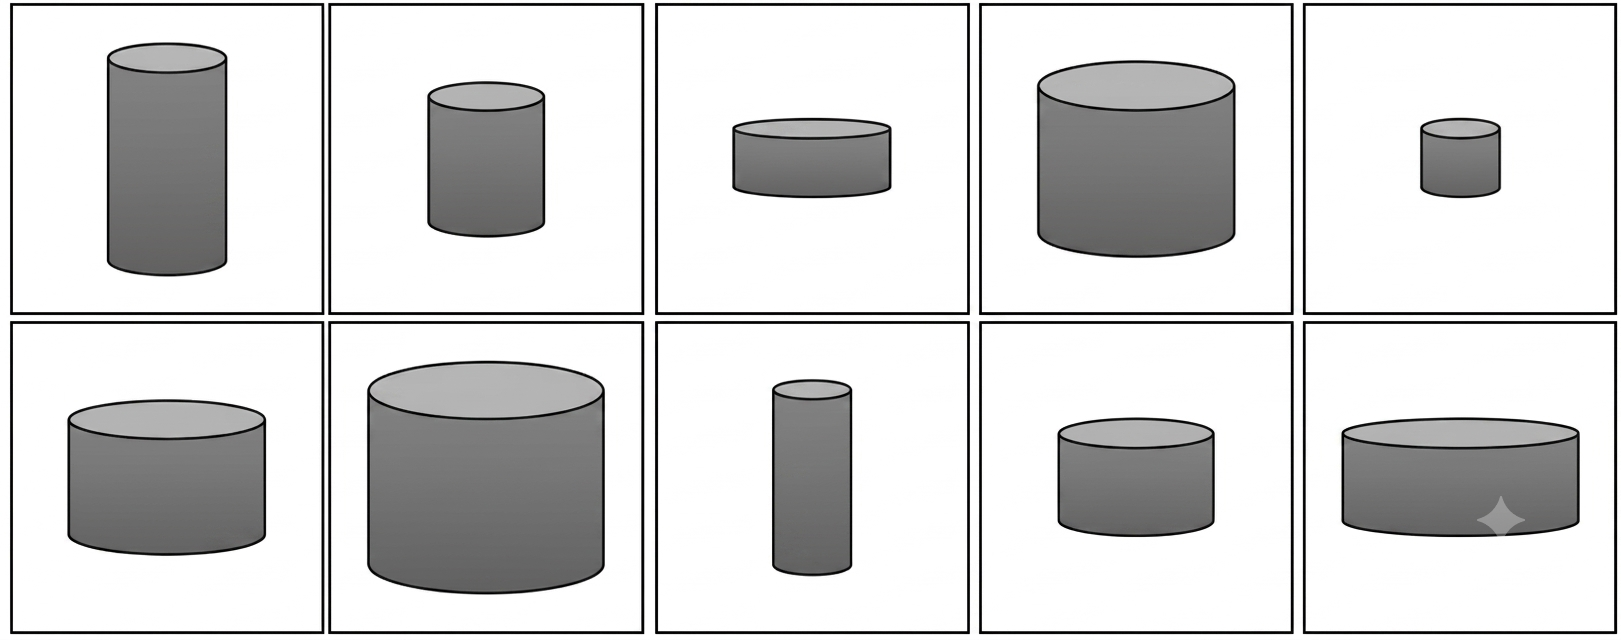
\includegraphics[width=\textwidth,height=0.85\textheight,keepaspectratio]{111.png}
			\caption{The biscuit tin dataset}
		\end{figure}
	\end{frame}
	
	\begin{frame}[plain]
		\begin{figure}
			\centering
			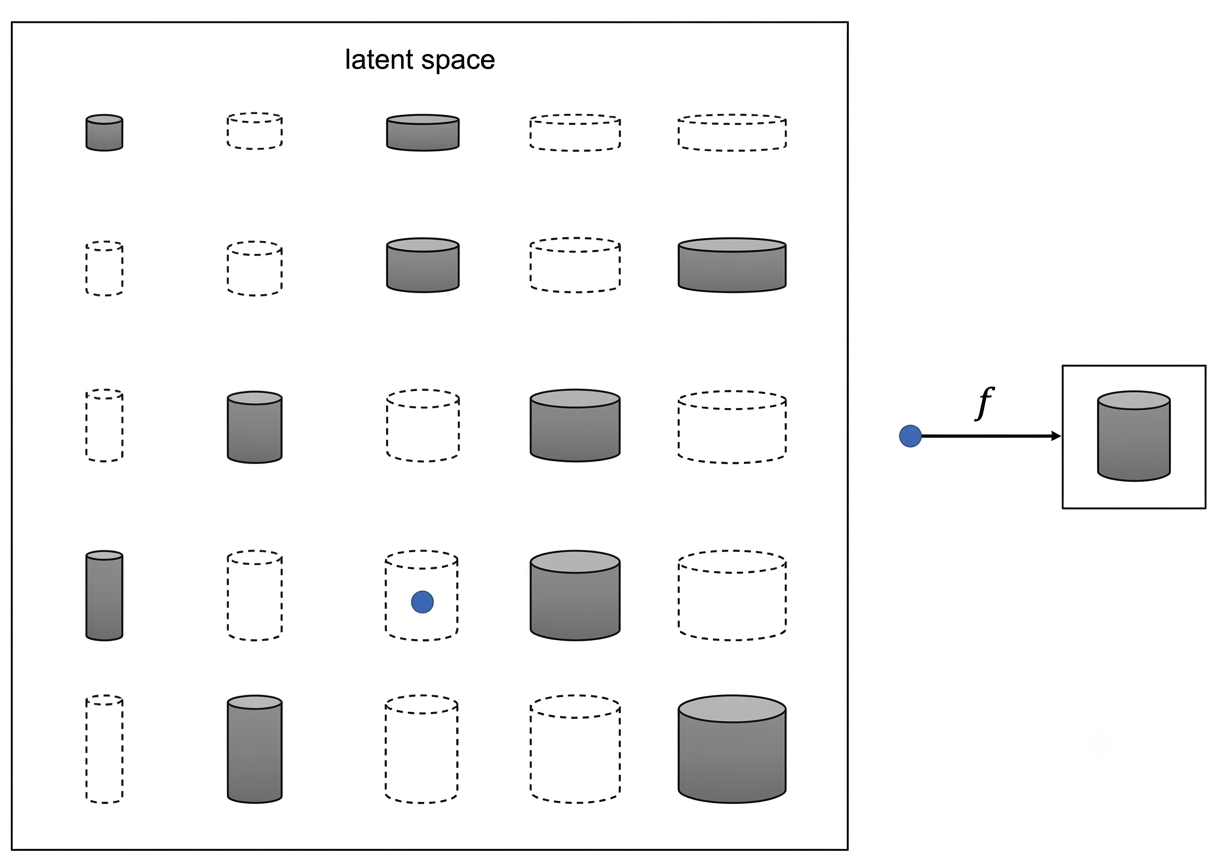
\includegraphics[width=\textwidth,height=0.85\textheight,keepaspectratio]{112.png}
			\caption{The latent space of biscuit tins and the function f that maps a point in the latent space to the original image domain}
		\end{figure}
	\end{frame}
	
	\begin{frame}[plain]
		\begin{figure}
			\centering
			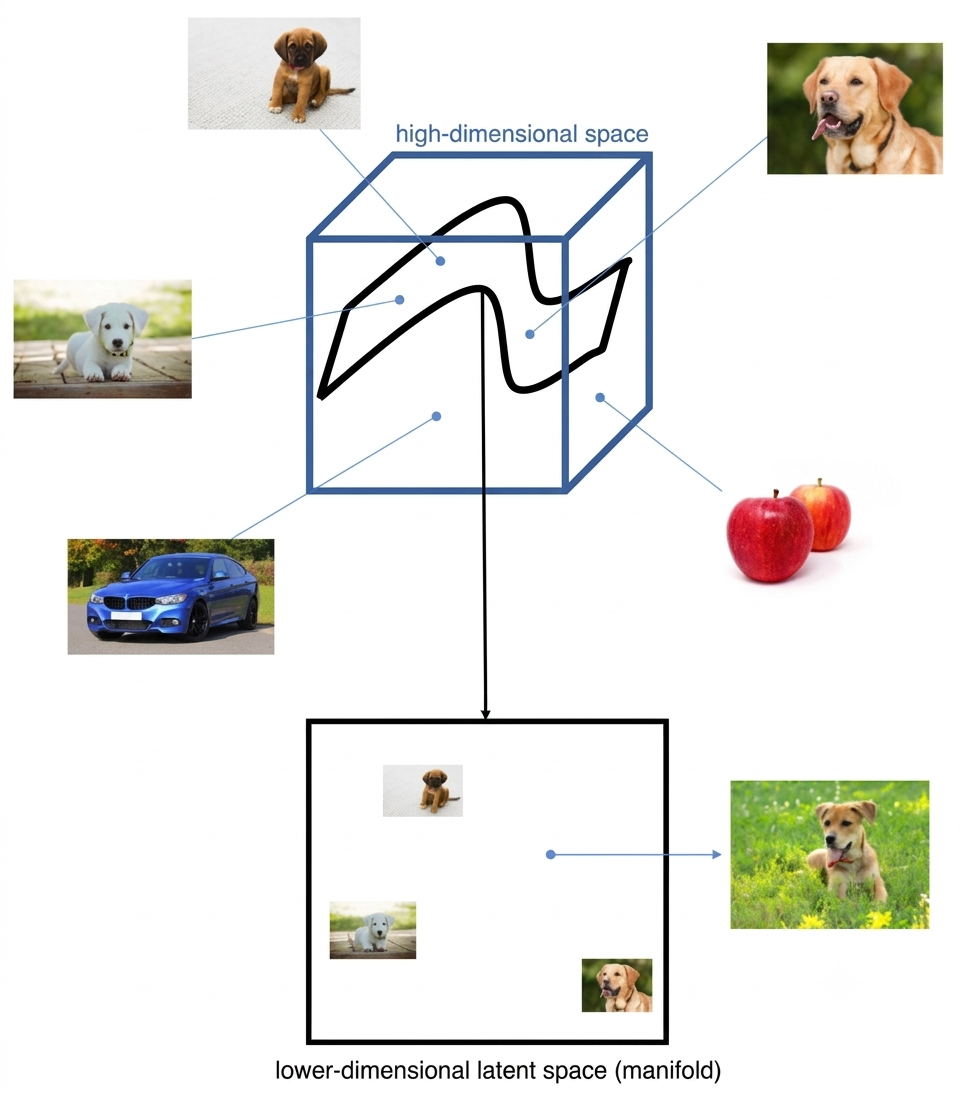
\includegraphics[width=\textwidth,height=0.75\textheight,keepaspectratio]{113.png}
			\caption{The cube represents the extremely high-dimensional space of all images; rep‐
				resentation learning tries to find the lower-dimensional latent subspace or manifold on
				which particular kinds of image lie (for example, the dog manifold)}
		\end{figure}
	\end{frame}
	
\end{document}